\chapter{Architecture and Technology Stack}
\label{ch:architecture}

\section{Background: Lambda and Kappa}
\label{sec:lit-lambda}

Lambda (Marz and Warren) combines an \emph{immutable master dataset}, a
\emph{batch layer} that recomputes exact views from it, and a \emph{speed
layer} that computes approximate views over recent data. Because batch
views are a pure function of immutable input, errors are repaired by
recomputing, and the speed layer's error is temporary by construction.
Kreps's critique is that Lambda needs two implementations of every
business rule, which can drift apart; his alternative, Kappa, keeps one
stream processor and recomputes by \emph{replaying the log}. That works
only if everything needed to recompute a result is \emph{in the log} ---
the assumption this use case breaks.

Three stream-processing results underpin the correctness argument:
event time (when something happened) must be separated from processing
time; a \textbf{watermark is a bet}, and events later than it are
dropped, not deferred; and Spark's exactly-once guarantee stops at the
sink, so external writes from \code{foreachBatch} are at-least-once
unless the sink is idempotent.

\section{The Decision: Lambda}
\label{sec:decision}

We implement Lambda: an archiver writes the immutable master dataset, a
speed layer computes live views, and a batch layer recomputes exact
views from the archive (Figure~\ref{fig:architecture}).

\begin{figure}[htbp]
\centering
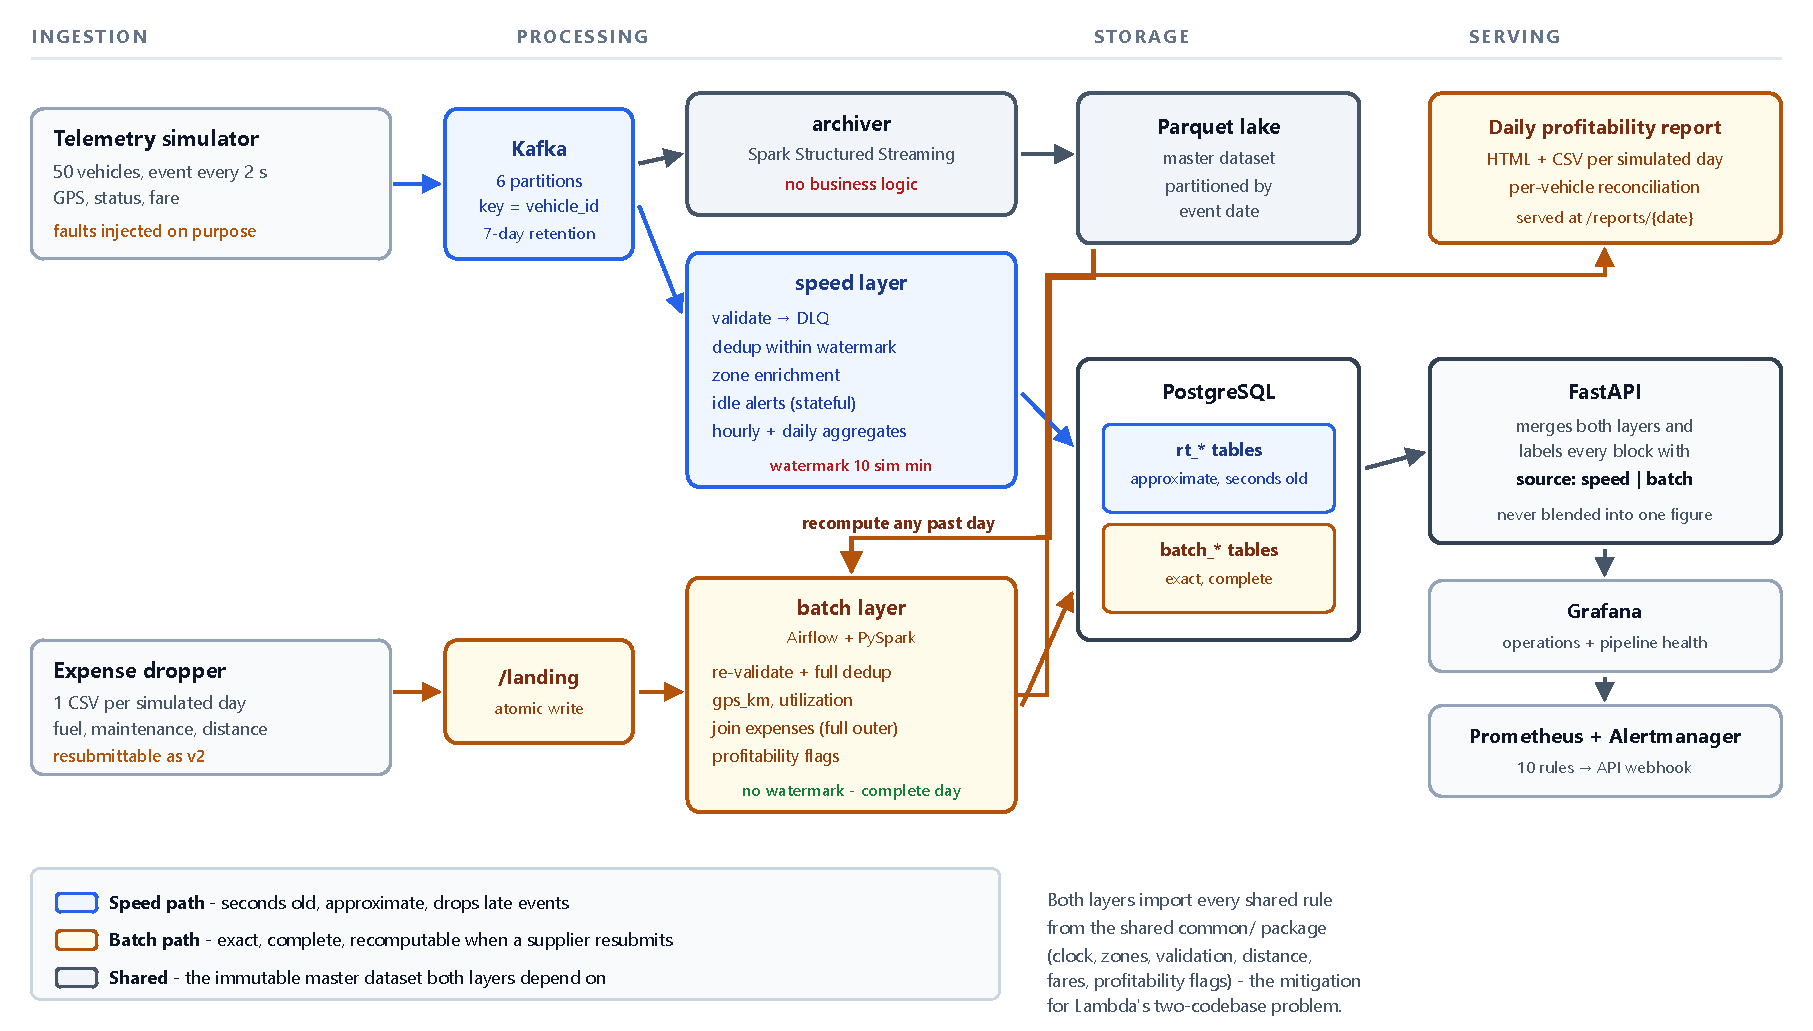
\includegraphics[width=0.95\textwidth]{figures/fig1-architecture.pdf}
\caption[System architecture]{System architecture. Blue: speed layer
(seconds old, approximate). Amber: batch layer (exact, recomputable).
Both read the same master dataset and import shared rules from
\code{common/}.}
\label{fig:architecture}
\end{figure}

\section{Why Kappa Was Rejected}
\label{sec:kappa-rejected}

The requirement is to \emph{restate a past day's financial figures} when
a partner sends corrected costs. Under Kappa:

\begin{enumerate}
  \item \textbf{Retention must cover any day we might restate} ---
        months of Kafka retention. Ours is \textbf{7 days}, enough for
        speed-layer recovery only.
  \item \textbf{Replay is not selective.} A Parquet lake partitioned by
        \code{sim\_date} lets the batch job read one partition; a full
        simulated day is computed in \textbf{9.4 seconds}.
  \item \textbf{The correction is not in the stream at all.} It arrives
        as a CSV file on a separate channel, so replaying the log does
        not touch what actually forces a restatement. Publishing the
        file to a topic only moves the problem back to point~1.
\end{enumerate}

A batch-only design was rejected because it cannot say which vehicles
are idle \emph{now}.

\section{What Lambda Costs, and Our Mitigation}
\label{sec:lambda-cost}

We accept Kreps's criticism and answer it structurally. A shared
\code{common/} package holds every rule both layers need --- simulated
clock, zone mapping, validation, haversine distance, fare maths and the
seven profitability flags --- and is imported by the simulators, both
processing layers and the API. Only two rules are duplicated, to avoid a
per-row Python UDF: validation (\code{validate\_event()} vs.\
\code{spark\_validation\_expr()}) and haversine distance. Each pair is
held in step by a test that feeds identical inputs to both.

\section{Technology Stack}
\label{sec:tech-stack}

Every image and package version is pinned (Table~\ref{tab:stack}).

\begin{table}[htbp]
\centering
\caption{Technology selection and the reason for each choice.}
\label{tab:stack}
\begin{tabularx}{\textwidth}{@{}llX@{}}
\toprule
\textbf{Layer} & \textbf{Choice} & \textbf{Why}\\
\midrule
Ingestion & Kafka 3.8 (KRaft) &
  Per-partition ordering is a correctness requirement; KRaft drops
  ZooKeeper.\\
Speed layer & Spark Structured Streaming 3.5.3 &
  Watermarks, windows and \code{applyInPandasWithState}; one engine for
  both layers makes \code{common/} shareable (preferred over Flink for
  that reason).\\
Master dataset & Parquet on a volume &
  Columnar, date-partitioned; paths built from \code{LAKE\_ROOT}, so
  moving to S3 is one variable.\\
Batch & Airflow 2.10 + PySpark &
  Retries, dependency ordering, per-task visibility; local mode suits
  $\sim$12k events/day.\\
Serving & PostgreSQL 16, FastAPI &
  Upserts on natural keys give idempotent sinks; Pydantic models make the
  \code{source} label part of the schema.\\
Observability & Prometheus, Alertmanager, Grafana &
  Pull-based metrics, routed alerts, dashboards.\\
\bottomrule
\end{tabularx}
\end{table}

\section{The Simulated Clock and Data Contract}
\label{sec:simclock}

\textbf{One real second is one simulated minute} (\code{COMPRESSION=60}),
so a simulated day takes 24 real minutes and a daily reconciliation can
be shown in a lab session. The clock is derived from a persisted start
instant, so every service agrees on \code{sim\_time} and restarts do not
rewind it.

We added three telemetry fields: \code{event\_id} (UUID, for
deduplication), \code{schema\_version}, and \code{event\_type}
(\code{ping}/\code{trip\_start}/\code{trip\_end}), which makes ``trips
completed'' a simple count instead of a chained stateful operator.
\textbf{\code{fare} is cumulative and final only on \code{trip\_end}}, so
revenue is \code{SUM(fare) WHERE event\_type='trip\_end'} in both layers.
